\documentclass[11pt,a4paper]{report}
\usepackage[utf8]{inputenc}
\usepackage[english]{babel}
\usepackage{amsmath}
\usepackage{hyperref}
\usepackage{breakurl}
\usepackage{amsfonts}
\usepackage{amssymb}
\usepackage{graphicx}
\begin{document}
%\maketitle
%Documentation for the car project
\section*{Embedded systems - Car project}
Johanna Vesterinen, Matthew Casserly, Carolina Lindqvist\\

\section*{Description}
The main schema for the car project can be seen in Fig. 1 \ref{car}. The main function in \verb|car.c| uses the functions that are defined in the \verb|control.*|,\verb|pid.*|, and \verb|display.*| files. The display is used as an output inside the for-loop.

\begin{figure}[h!]
\label{car}
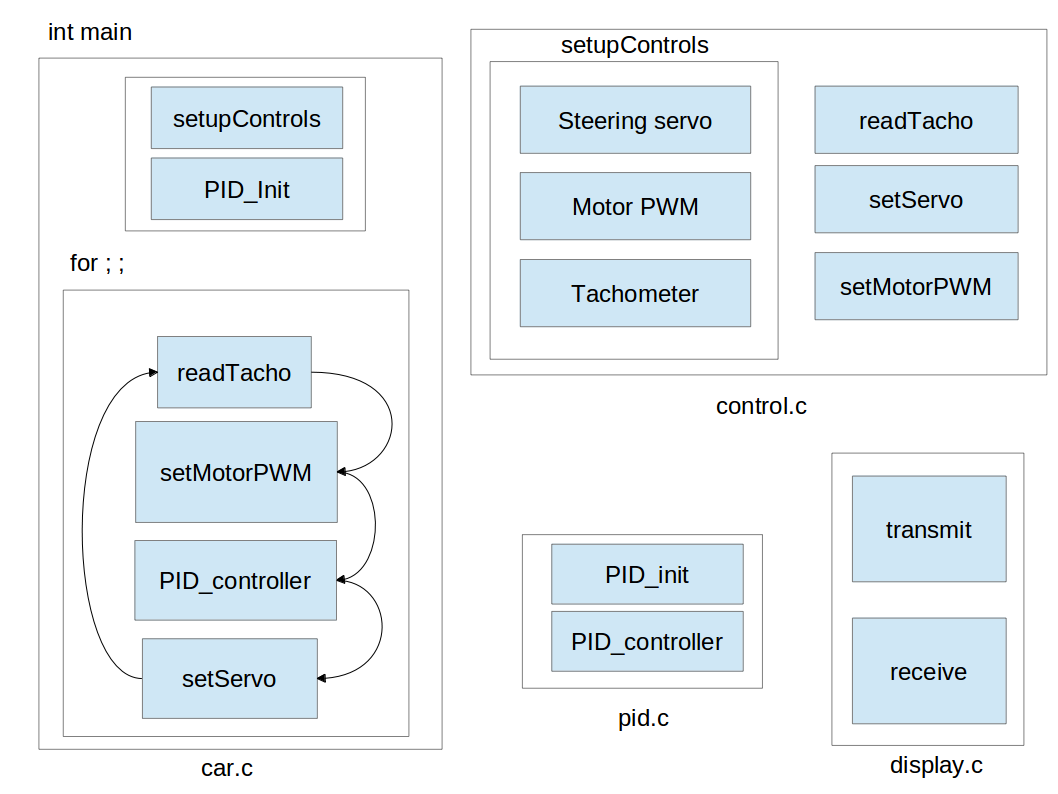
\includegraphics[scale=0.45]{car-schema.png}
\caption{Car project plan}
\end{figure}

\section*{Chosen settings}
The steering servo uses the Fast PWM mode with the prescaler value 8. It uses the set at bottom and "clear at match" settings. 
The motor PWM has the prescaler 1. Tachometer reading is done by an interrupt that regulates the motor PWM based on the readouts. The timer interrupt uses a \/64 prescaler. All prescaler values were chosen based on how well they fit with the 16 MHz clock, e.g. in order to regulate how often the tachometer readings updates (corrects) the speed. The PID values are chosen based on what seemed suitable for the car on the test track.

\section*{Files}
\subsubsection*{car.*}
The \verb|car.c| file contains the main for-loop that reads the steering sensors and adjusts the steering according to the sensor readings. First the initial PID values are set and the controller logic (timers, interrupts, modes...) is set up. During run, the TIMER3\_COMPA\_vect interrupt adjusts the PID interval, i.e. how often the sensors are read and the speed and direction adjusted. The \verb|car.c| file also contains the initial PID values. Both the motor and the steering have their own controller.

Inside the for-loop the tachometer is read and the PID controller is used to calculate a new value for the motor PWM and the servo. These new values are set and some of the values are printed on the display. A "start" button logic is included - the for-loop starts executing as the black button is pressed.


\subsubsection*{control.*}
The \verb|control.*| files contain the logic for regulating the speed and adjusting the direction the car travels in. The AVR chip configuration commands are also included (interrupts, timers, PWM, USART...) in the setupControls function. All eight sensors are read by the readSensors function. The functionality for setting the speed and reading the tachometer are also defined in \verb|control.*|.

\subsubsection*{pid.*}
In \verb|pid.*| the PID control algorithm is defined based on the implementation from ATMEL AN221. The implementation contains an initialization function for the start values, and a PID control algorithm.

\subsubsection*{display.*}
These files contain the control logic for the display. Input can be sent and received. There are separate functions for printing strings, integers, and clearing the screen. It is based on the USART functionality from the AVR standard IO library.%t

\end{document}
